%%Relacionar mejor el inicio de este capítulo en relación a lo escrito en la introducción. Lo de ahorita es, en principio, preliminar. 

%El objetivo de esta tesis es sacarle todo el provecho posible al transporte de jets y los indicadores que éste nos pueda regalar. Por esto, dos problemas físicos sencillos pero interesantes serán desarrollados en esta sección. El primero es el \textit{problema restringido de 3 cuerpos en una órbita circular (PR3COC)} y el segundo el \textit{sistema de Henón-Heiles (SHH)}. Antes de entrarle de lleno a estos problemas, creo que vale la pena recapitular un poco sobre la teoría en la que están basados; la mecánica analítica. Este capítulo se desarrollará como sigue: primero se hará un repaso de la mecánica lagrangiana y hamiltoniana muy al estilo de Landau y Lifshitz, específicamente en los capítulos I,II y VII de \cite{mechanics_landau_lifshitz}, luego, se desarrollará la teoría de PR3COC y, finalmente la de SHH.

\section{Problema de tres cuerpos sin restricciones}
\label{sec:3BP}

El problema de tres cuerpos interactuando en campos gravitacionales ha sido uno de gran controversia desde hace más de 300 años ya que la dinámica de éste tiene comportamientos que distan de ser obvios. Aún en el caso más simplificado, o sea, el caso restringido de tres cuerpos en órbitas circulares (PR3COC), el problema presenta alta sensibilidad a las condiciones iniciales, varios puntos de equilibrio, órbitas periódicas y semiperiódicas y, en general, una rica dinámica. Además,el PR3COC tiene únicamente dos grados de libertad (en vez de los 18 del problema general de tres cuerpos) lo cuál permite un estudio y una representación gráfica mucho más alcanzable respecto al problema original. En este sentido, se antoja analizar dicha dinámica con las herramientas desarrolladas en \ref{chap:jt_indicators}.

Adicionalmente, el apéndice \ref{chap:mecanics} tiene un repaso general de la mecánica analítica, de la cual se basa el plantemiento de este problema. 

El problema es planteado con el potencial gravitacional de Newton entre pares de cuerpos 
\begin{align}
 U_{M_1}(\mathbf{r}_1,\mathbf{r}_2,\mathbf{r}_3) &= -G \frac{M_1 M_2}{r_{1,2}} - G \frac{M_1 M_3}{r_{1,3}} \\
 U_{M_2}(\mathbf{r}_1,\mathbf{r}_2,\mathbf{r}_3) &= -G \frac{M_2 M_1}{r_{2,1}} - G \frac{M_2 M_3}{r_{2,3}} \\
 U_{M_3}(\mathbf{r}_1,\mathbf{r}_2,\mathbf{r}_3) &= -G \frac{M_3 M_1}{r_{3,1}} - G \frac{M_3 M_2}{r_{3,2}}
 \label{eq:3body_potential}
\end{align}

con $G$ la constante de gravitación universal, $\mathbf{r}_i = x_i \hat{\imath} + y_i \hat{\jmath} + z_i \hat{k}$ la posición de la i-ésima partícula, $M_i$ su masa y $r_{i,j} = \norm{ \mathbf{r}_i - \mathbf{r}_j}$ la distancia entre las partículas $M_i$ y $M_j$\footnote{Notemos la simetría $r_{i,j} = r_{j,i}$, aunque $\mathbf{r}_{i,j} = \mathbf{r}_i - \mathbf{r}_j = \mathbf{r}_j - \mathbf{r}_i  = - \mathbf{r}_{j,i}$.}. 

La energía cinética del problema la definimos de la manera usual 
\begin{equation}
 T(\dot{\mathbf{r}}_1,\dot{\mathbf{r}}_2,\dot{\mathbf{r}}_3) = \sum_{i=1}^3 M_i \dot{r}_i^2,
 \label{eq:3body_cinetic}
\end{equation}
lo cual define un sistema de 6 ecuaciones de movimiento dadas por (\ref{eq:newton_second_law})
\begin{equation}
 M_i \ddot{\mathbf{r}_1,\mathbf{r}_2,\mathbf{r}_3} = - G M_i \sum_{j\neq i} \frac{M_j}{r_{i,j}^2} \hat{\mathbf{r}}_{i,j},
 \label{eq:3body_eqs_motion}
\end{equation}
con $\hat{\mathbf{r}}_{i,j} = \frac{\mathbf{r}_{i,j}}{r_{i,j}}$ un vector unitario en la dirección de $\mathbf{r}_{i,j}$.

Éste es el caso más general del problema de tres cuerpos ya que ninguna restricción ha sido impuesta hasta el momento. Sin embargo, para el problema \textbf{restringido} de tres cuerpos uno supone que una de las partículas tiene una masa tan baja que no afecta a las otras dos y, por esto, las dos más grandes se mueven como si la tercera no existiera. Vale la pena estudiar primero el caso de dos cuerpos, ver la dinámica entre las dos partículas más masivas y luego regresar a estudiar el movimiento de la tercer partícula bajo la influencia de estas dos. 

\section{Problema de dos cuerpos}
\label{sec:2body_problem}
Dadas que $M_1$ y $M_2$ son los cuerpos de mayor masa o \textbf{primarios} y $m_3$ es despreciable, la dinámica de dichos cuerpos queda definida por
\begin{equation}
 \mathbf{F}_1(\mathbf{r}_1,\mathbf{r}_2) = M_1 \ddot{\mathbf{r}}_1 = -G \frac{M_1 M_2}{r_{1,2}^2} \hat{\mathbf{r}}_{1,2}.
 \label{eq:2body_eqs_motion}
\end{equation}
Como $\hat{\mathbf{r}}_{1,2} = - \hat{\mathbf{r}}_{2,1}$ entonces $\mathbf{F}_2 = -\mathbf{F}_1$, lo cual es equivalente a la tercera ley de Newton. Se tomará como referencia el capítulo 3 del Goldstein \cite{Goldstein2007} para obtener las soluciones de este problema. Por comodidad llamaremos a $\mathbf{r}_{1,2}$ simplemente $\mathbf{R}$ y, en términos de ésta, se puede plantear el problema de Kepler, que describe la aceleración relativa
\begin{equation}
 \ddot{\mathbf{R}} = \ddot{\mathbf{r}}_1 - \ddot{\mathbf{r}}_2 = -G \frac{M_1 + M_2}{R^2} \hat{\mathbf{R}} = - \frac{\beta}{R^2}\hat{\mathbf{R}}
 \label{eq:kepler_problem}
\end{equation}
con $\beta = G \left(M_1 + M_2 \right)$. Multiplicando (\ref{eq:kepler_problem}) por $\gamma := \frac{M_1 M_2}{M_1+M_2}$ obtenemos las ecuaciones de movimiento de la fuerza relativa de $M_1$ respecto a $M_2$ como si $M_2$ estuviera fija y $M_1$ tuviera masa reducida $\gamma$.

El problema de Kepler conserva el momento angular $\mathbf{L} := \mathbf{R} \times \mathbf{p}$, ya que
\begin{equation}
 \frac{d\mathbf{L}}{dt} = \frac{d}{dt}\left(\mathbf{R} \times \gamma\dot{\mathbf{R}} \right) = \gamma\dot{\mathbf{R}} \cancelto{0}{\times}\dot{\mathbf{R}} + \mathbf{R} \times \gamma \ddot{\mathbf{R}} = - \mathbf{R} \cancelto{0}{\times} G\frac{\gamma \beta}{r^2}\hat{\mathbf{R}} = 0
\end{equation}
y, por tanto, $\mathbf{L} = \text{constante}$. Como primera consecuencia $\mathbf{R}$ y $\dot{\mathbf{R}}$ son perpendiculares a $\mathbf{L}$ y por tanto, viven en un plano. Por comodidad se escogerá un eje coordenado tal que dicho plano esté sobre $xy$. 

Una mejor descripción del movimiento se puede obtener en coordenadas polares, donde
\begin{align}
 \hat{R} &= \cos \theta \hat{\imath} + \sin \theta \hat{\jmath} \nonumber \\
 \hat{\theta} &= -\sin \theta \hat{\imath} + \cos \theta \hat{\jmath}
 \label{eq:polar_transformation}
\end{align}
y $z$ ya no necesita descripción ya que $z=0$ para toda la trayectoria. 

Debemos encontrar ahora las expresiones de $\mathbf{R}$,$\dot{\mathbf{R}}$ y $\ddot{\mathbf{R}}$ para replantear las ecuaciones de movimiento del sistema. Haciendo regla de la cadena obtenemos
\begin{align}
 \mathbf{R} &= R \cos \theta \hat{\imath} + R \sin \theta \hat{\jmath} = R \hat{R} \\
 \dot{\mathbf{R}} &= \left( \dot{R} \cos \theta - R \sin \theta \dot{\theta} \right) \hat{\imath} + \left( \dot{R} \sin \theta + R \cos \theta \dot{\theta} \right) \hat{\jmath} = \dot{R}\hat{R} + R \dot{\theta} \hat{\theta} \\
 \ddot{\mathbf{R}} &= \left(\ddot{R} - R \dot{\theta}^2 \right) \hat{R} + \left( R \ddot{\theta} + 2 \dot{R}\dot{\theta} \right) \hat{\theta}.
 \label{eq:motion_polar_variables}
\end{align}

De hecho, en éste sistema de coordenadas es fácil ver que
\begin{equation}
 L = \norm{ \mathbf{L} } = \norm{ \mathbf{R} \times \gamma \dot{\mathbf{R}} } = \norm{ \left( R \hat{R} + 0 \hat{\theta} + 0 \hat{k} \right) \times \left( \dot{R} \hat{R} + R \dot{\theta} \hat{\theta} + 0\hat{k} \right) } = \gamma R^2 \dot{\theta}
\end{equation}
para encontrar una expresión para la velocidad angular 
\begin{equation}
\dot{\theta}(R) = \frac{L}{\gamma R^2}.
\label{eq:2body_ang_vel}
\end{equation}

Ahora, con (\ref{eq:motion_polar_variables}) podemos replantear (\ref{eq:kepler_problem}) y obtener las ecuaciones de movimiento en las nuevas coordenadas
\begin{align}
 R \ddot{\theta} + 2 \dot{R} \dot{\theta} &= 0 \\
 \ddot{R} - R \dot{\theta}^2 &= -\frac{\beta}{R^2}.
 \label{eq:2body_eqs_motion_polar}
\end{align}
Notemos que la primera queda resuelta por (\ref{eq:2body_ang_vel}) mientras que la segunda, notando la relación $\dot{R} = \frac{d R}{d\theta} \dot{\theta}$, se convierte en
\begin{align*}
 \frac{d^2 R}{d \theta^2} \dot{\theta}^2 + \frac{dR}{d\theta} \ddot{\theta} - R \dot{\theta}^2 = - \frac{\beta}{R^2}
\end{align*}
donde 
\begin{equation*}
 \ddot{\theta} = -\frac{2L}{\gamma R^3}\dot{R} = -\frac{2L}{\gamma R^3} \frac{dR}{d\theta}\dot{\theta} = - \frac{2L^2}{\gamma^2 R^5} \frac{dR}{d\theta}.
\end{equation*}
Ésto y (\ref{eq:2body_ang_vel}) se sustituyen en  (\ref{eq:2body_eqs_motion_polar}) para obtener
\begin{equation*}
 \frac{L^2}{\gamma^2 R^4}\left( \frac{d^2R}{d\theta^2} - \frac{1}{R} \left(\frac{dR}{d\theta} \right)^2 -R \right) = - \frac{\beta}{R^2}.
\end{equation*}

Finalmente, si hacemos $u(R) := \frac{1}{R}$, se simplifica la ecuación diferencial a
\begin{equation}
 \frac{d^2u}{d\theta^2} + u = \frac{\beta \gamma^2}{L^2},
\end{equation}

que no es más que un oscilador armónico con forzamiento constante $\frac{\beta \gamma^2}{L^2}$. Obtenemos explícitamente la solución para $u$:

\begin{equation*}
 u(\theta) = \frac{\beta \gamma^2}{L^2} \left( 1 + e \cos (\theta - \theta_0 ) \right) 
\end{equation*}
\begin{equation}
 \therefore R(\theta) = \frac{L^2}{\beta \gamma^2 \left(1 + e \cos (\theta - \theta_0) \right)}.
 \label{eq:2body_solution}
\end{equation}

%Cómo obtenemos explícitamente la forma de $e$ y de $\theta_0$? 
%Por qué esta ecuación representa una sección cónica en polares? Debería simplemente decirlo y citar algún texto? Chance sí...  

Ésta es la distancia relativa que tienen $M_1$ y $M_2$ en función del ángulo $\theta$. Notemos que (\ref{eq:2body_solution}) representa diferentes secciones cónicas en coordenadas polares y depende de la eccentricidad $e$ que tenga. 

\section{Problema restringido de 3 cuerpos en una órbita circular (PR3COC)}

Es ahora que estamos en posición de empezar a poner constricciones al problema de los tres cuerpos. 

Como ya se había mencionado, supondremos que la tercer partícula será mucho más pequeña que las otras dos, i.e., $m_3 \ll M_2 \leq M_1$. Así, la consecuencia principal es que $m_3$ no afecta la dinámica de $M_2$ ni de $M_1$ y, por tanto, la solución para los cuerpos primarios es la desarrollada en \ref{sec:2body_problem}. Sólo queda por estudiar la dinámica de $m_3$.

Para restringir las órbitas a que sean circulares es necesario imponer que $R(\theta)$ tenga eccentricidad $e=0$; así
\begin{equation}
 R = \frac{L^2}{\gamma^2 \beta}.
 \label{eq:3body_restricted_solution}
\end{equation} 

Con esto, podemos dar una expresión para la velocidad angular que no dependa del momento angular $L$, es decir, con (\ref{eq:3body_restricted_solution}) en (\ref{eq:2body_ang_vel}) se obtiene
\begin{equation}
 \Omega := \dot{\theta} = \sqrt{ \frac{\beta R}{R^4} } = \sqrt{\frac{G \left(M_1 + M_2 \right)}{R^3}}.
 \label{eq:3body_ang_velocity}
\end{equation}
Notemos que al estar restringido el movimiento a órbitas circulares $R$ es constante en todo momento y por ello la velocidad angular también.

Para trabajar la dinámica de $m_3$ conviene establecer un marco de referencia en rotación de modo que $M_1$ y $M_2$ estén en reposo. Dicha rotación tendrá velocidad angular $\Omega$ y estará basada en el centro de gravedad entre las dos. Recordemos, de la sección \ref{sec:ficticious_forces}, que un sistema de referencia en rotación traerá algunas fuerzas ficticias descritas por (\ref{eq:rotating_constant_acceleration}), más específicamente la aceleración de Coriolis y la aceleración centrípeta. Como en este caso el sistema está centrado en el centro de gravedad de $M_1$ y $M_2$, la aceleración inercial del sistema será nula en todo momento.

Las ecuaciones de movimiento para $m_3$ en este sistema quedan descritas como
\begin{equation}
 \ddot{\mathbf{r}} + 2\mathbf{\Omega} \times \dot{\mathbf{r}} = - \nabla V(\mathbf{r})
 \label{eq:3body_restricted_acceleration}
\end{equation}
con $\mathbf{r} = (x,y,z)$ la distancia de $m_3$ al centro de gravedad, $\mathbf{R} = \mathbf{r}_1 - \mathbf{r}_2 = (r_1 + r_2,0,0)$ la distancia entre $M_1$ y $M_2$ y
\begin{equation}
 V(r) = \left( -G \frac{M_1}{\norm{\mathbf{r}-\mathbf{r_1}}} - G \frac{M_2}{\norm{\mathbf{r}-\mathbf{r_2}}} - \frac{1}{2} \Omega^2 r^2 \right)
 \label{eq:3body_restricted_potential}
\end{equation} 
la parte cerrada del potencial, que se suele conocer como \textbf{pseudo-potencial}, ya que si la velocidad es distinta de cero, la fuerza de Coriolis debe ser considerada para la dinámica de la partícula.

Con el afán de reducir el número de parámetros que definen al problema, trabajaremos en unidades especiales tales que 
\begin{align}
 M_1 + M_2 &= 1 \ um \nonumber \\
 R = r_2 - (-r_1) &= 1 \ ud \nonumber \\
 \Omega &= 1 \frac{rad}{ut} \nonumber \\
 \implies G &= 1 \frac{ud^3}{ut^2 \cdot um},
 \label{eq:3body_new_units}
\end{align}
Éstas nos permiten además adimensionalizar las ecuaciones de movimiento. Para esto, es cómodo poner el origen en el centro de masa entre $M_1$ y $M_2$, y a éstas alineadas sobre el eje $x$, así $CM = (0,0) = (\frac{-M_1r_1 + M_2r_2}{M_1 + M_2}, 0)$ obteniendo $-r_1 = -\frac{M_2}{M_1+M_2}R$ y $r_2 =\frac{M_1}{M_1+M_2}R$. Definimos el parámetro de masa 
\begin{equation*}
 \mu = \frac{M_2}{M_1 + M_2} 
\end{equation*}
con el que podemos replantear todo en términos adimensionales
\begin{align}
 M_1 &= 1 - \mu \nonumber \\
 M_2 &= \mu \nonumber \\
 -r_1 &= -\mu \nonumber \\
 r_2 &= 1 - \mu \nonumber \\
 G &= 1 \nonumber \\
 \Omega &= 1
 \label{eq:3body_adimensional_units}
\end{align}
tomando en cuenta las cantidades de (\ref{eq:3body_new_units}).

Así, (\ref{eq:3body_restricted_potential}) se expresa como
\begin{equation}
 V(r) = V(x,y) = -\frac{1 - \mu}{\sqrt{(x + \mu)^2 + y^2}} -  \frac{\mu}{\sqrt{(x - 1 + \mu)^2 + y^2}} - \frac{1}{2} \left(x^2 + y^2 \right)
\end{equation}
con las ecuaciones de movimiento asociadas a (\ref{eq:3body_restricted_acceleration})
\begin{align}
 \dot{x} &= v_x \\
 \dot{y} &= v_y \\
 \dot{v}_x - 2v_y &=  x - \frac{(1 - \mu) (x+\mu)}{\sqrt{ (x+\mu)^2 + y^2 }^3} - \frac{\mu (x - 1 + \mu) }{\sqrt{(x - 1 +  \mu)^2 + y^2}^3 } \\ 
 \dot{v}_y + 2v_x &= y \left( 1 - \frac{ 1 - \mu }{\sqrt{(x+\mu)^2 + y^2}^3} - \frac{\mu}{\sqrt{(x - 1 + \mu)^2 + y^2}^3} \right),
 \label{eq:3body_restricted_ eqs_motion}
\end{align}
donde todo queda en términos del único parámetro $\mu$.

Existe una primera integral del sistema si hacemos el producto interno de (\ref{eq:3body_restricted_acceleration}) por $\dot{\mathbf{r}}$, que resulta en 
\begin{align*}
 \ddot{x} \dot{x} + \ddot{y} \dot{y} &= - \pder{V}{x}\dot{x} - \pder{V}{y} \dot{y} \\
 \implies - \frac{1}{2} \left( \dot{x}^2 + \dot{y}^2 \right) &= \int \frac{d V}{dt} = V - C_J 
\end{align*}
\begin{equation}
 \therefore C_J = V + \frac{1}{2}v^2,
 \label{eq:3body_jacobi_constant}
\end{equation}
con $C_J$ la constante de integración que se conoce como \textbf{constante de Jacobi} o \textbf{energía de Jacobi}.

\subsection{Puntos lagrangianos}
\label{sec:lag_points}

Aún sin ser conservativo, vale la pena estudiar las curvas de nivel de pseudo-potencial ya que éste nos dará una buena intuición sobre cómo será la trayectoria de nuestra partícula. De hecho, los puntos singulares que puedan aparecer seguirán siéndolo cuando se tome en cuenta la aceleración de Coriolis. La figura \ref{fig:3body_pseudo_potential} presenta dichas curvas de nivel, donde se observan tres puntos singulares en el eje alineados a $M_1$ y $M_2$ que se suelen llamar $L_2$,$L_1$ y $L_3$, respectivamente. Otros dos puntos existen para $y \neq 0$ los cuales se conocen como $L_4$ y $L_5$. Éstos cinco reciben el nombre de \textit{puntos lagrangianos} en honor a los estudios de Joseph Lagrange sobre el tema.

%FIGURA! 
\begin{figure}[h!]
 \centering
 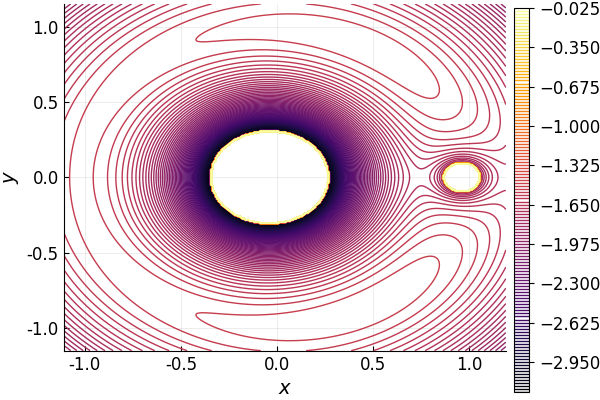
\includegraphics[width=0.8\linewidth]{pseudo_potential}
 \caption{Curvas de nivel para el pseudo-potencial $V(x,y)$ con $M_1 = 26M_2$, $R = 10$ Y $G=1$ en unidades adimensionales.}
 \label{fig:3body_pseudo_potential}
\end{figure}

Siguiendo el desarrollo de \cite{Cornish1998, Windall2008}, encontraremos dónde están dichos puntos singulares y se hará un análisis de estabilidad de éstos.

Los tres primeros se dan cuando $y=0$, quedando por resolver únicamente cuándo $\dot{v}_x = 0$. Esto plantea una ecuación de quinto grado en $x$ complicada de resolver analíticamente. Sin embargo, cuando $M_1$ es considerablemente más grande que $M_2$, se puede tomar la aproximación a primer orden de $\mu$ y conseguir
\begin{align}
 L_1 &\approx \left( \left[ 1 - \left(\frac{\mu}{3}\right)^{1/3} \right] R , 0 \right) \nonumber \\ 
 L_2 &\approx \left( R\left[ 1 + \left(\frac{\mu}{3}\right)^{1/3} \right] R , 0 \right) \nonumber \\
 L_3 &\approx \left( -R\left[ 1 5 \frac{5 \mu}{12} \right] R, 0 \right).
 \label{eq:3body_L123}
\end{align} 

También se pueden obtener estos valores numéricamente para cualquier $\mu$, pero hace un poco más complicado el análisis de estabilidad ya que no se consiguen en función de $\mu$. Sin embargo, como se observa en la figura \ref{fig:3body_pseudo_xaxis}, para $\mu = \frac{1}{27}$ sí se llega a notar la diferencia.

%FIGURA!
\begin{figure}[h!]
 \centering
 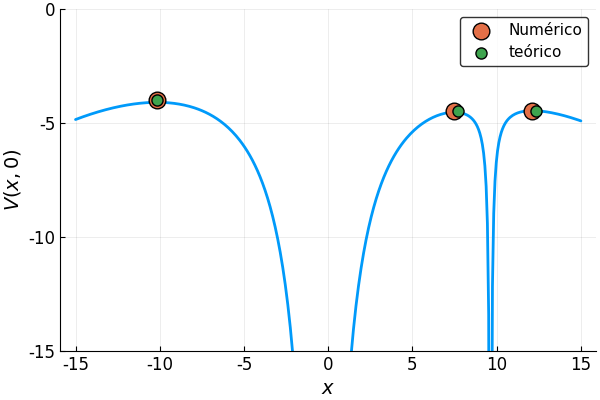
\includegraphics[width=0.8\linewidth]{pseudo_xaxis}
 \caption{Proyección del pseudo-potencial en el eje $x$ para ver sus puntos de inflexión. Aparecen $L_1, L_2$ y $L_3$ calculados con (\ref{eq:3body_L123}) (verde) y numéricamente (naranja).}
 \label{fig:3body_pseudo_xaxis}
\end{figure}

Para obtener $L_4$ y $L_5$ es importante destacar que la fuerza centrípeta es, por definición, radial hacia afuera. En este sentido, en la dirección radial se deben balancear la fuerza centrípeta con la gravitacional. Esto hace que el balance en la dirección tangencial sea debido únicamente a los dos objetos masivos interactuando bajo sus campos gravitacionales. Para obtener esto, hacemos una proyección de la fuerza hacia sus direcciones radiales y tangenciales con los vectores $\mathbf{r}_{\parallel} = (x,y)$ y $\mathbf{r}_{\bot} = (-y,x)$, así
\begin{align*}
 F_{\bot} &= \frac{1}{r_{\bot}} \mathbf{r}_{\bot} \cdot \mathbf{F} = \frac{y}{r_{\bot}} \left( - \frac{(1-\mu)(x + \mu)}{ r_{1,3}^3 } - \frac{\mu(x - 1 +\mu )}{ r_{2,3}^3 } + \frac{(1-\mu)x}{ r_{1,3}^3 } + \frac{\mu x}{ r_{2,3}^3 } \right) \\
 \therefore F_{\bot} &= \frac{ \mu(1-\mu) y}{r_{\bot}} \left( \frac{1}{r_{1,3}^3} - \frac{1}{r_{2,3}^3} \right),
\end{align*}
es decir, la condición para que la componente tangencial de la fuerza se anule es que ambos cuerpos estén a la misma distancia de la partícula $m_3$, lo cual tiene sentido ya que el sistema tiene el origen en el centro de masa entre $M_1$ y $M_2$. 

Para la componente radial, tenemos que
\begin{align*}
 F_{\parallel} &= \frac{1}{r_{\parallel}} \mathbf{r}_{\parallel} \cdot \mathbf{F} = \frac{1}{r_\parallel} \left( (x^2 + y^2) -  (1-\mu) \left( \frac{(x+ \mu)x}{r_{1,3}^3} + \frac{y^2}{r_{1,3}^3} \right) - \mu \left( \frac{(x - 1 +\mu) x}{r_{2,3}^3} + \frac{y^2}{r_{2,3}^3} \right) \right),
\end{align*}
pero $r_{1,3} = r_{2,3}$, por lo que lo anterior se simplifica a 
\begin{align*}
 F_{\parallel} = \frac{x^2 + y^2}{r_\parallel} \left( \frac{1}{R^3} - \frac{1}{r_{1,3}^3} \right).
\end{align*}

Encontramos que $r_{1,3} = r_{2,3} = R$. $L_4$ y $L_5$ forman un tríangulo equilátero de lado $R$, cuya base es la distancia entre $M_1$ y $M_2$. Así,
\begin{align}
 L_4 &= \left( \frac{1 - 2\mu}{2}, \frac{\sqrt{3}}{2} \right) \\
 L_5 &= \left( \frac{1 - 2\mu}{2} , -\frac{\sqrt{3}}{2} \right)
 \label{eq:L4_L5}
\end{align} 
tal como se ve en la figura \ref{fig:L_diagram}.

%FIGURA! 

La estabilidad de estos puede estudiarse viendo cómo se comportan las ecuaciones de primera variación alrededor de los puntos de equilibrio, tal como se hace en \cite{Cornish1998}. Para esto basta construir la matriz de estabilidad 
\begin{equation*}
 A(\mathbf{x}) = \begin{bmatrix}
  \pder{\mathbf{f}_1}{x_1}(\mathbf{x}) & \dots & \pder{\mathbf{f}_1}{x_n}(\mathbf{x}) \\
  \vdots & \ddots & \vdots \\ 
  \pder{\mathbf{f}_n}{x_1}(\mathbf{x}) & \dots & \pder{\mathbf{f}_n}{x_n} (\mathbf{x})
\end{bmatrix}
\end{equation*}
donde $\dot{\mathbf{x}} = \mathbf{f}(\mathbf{x})$ y encontrar los eigenvalores de ésta para determinar qué tipo de punto singular se trata. Para éste caso
\begin{equation}
 A(\mathbf{x}_{L_i}) = \begin{bmatrix}
  0 & 0 & 1 & 0 \\
  0 & 0 & 0 & 1 \\ 
  \pder{\dot{v_x}(\mathbf{x}_{L_i})}{x} & \pder{\dot{v_x}(\mathbf{x}_{L_i})}{y} & 0 & 2 \Omega \\
  \pder{\dot{v_y}(\mathbf{x}_{L_i})}{x} & \pder{\dot{v_y}(\mathbf{x}_{L_i})}{y} & -2\Omega & 0
\end{bmatrix}
\end{equation}
representa dicha matriz, y ésta será evaluada en los puntos lagrangianos $\mathbf{x}_{L_i}$, donde 
\begin{align}
 \pder{\dot{v}_x}{x} &=  1 - \frac{1-\mu}{r_{1,3}^3} + 3\frac{(1-\mu)(x + \mu)^2}{r_{1,3}^5} - \frac{\mu}{r_{2,3}^3} + 3\frac{\mu(x - 1 + \mu)^2}{r_{2,3}^5} \nonumber \\ 
 \pder{\dot{v}_y}{y} &= 1 - \frac{1-\mu}{r_{1,3}^3} + 3\frac{(1-\mu)y^2}{r_{1,3}^5} - \frac{\mu}{r_{2,3}^3} + 3\frac{\mu y^2}{r_{2,3}^5} \nonumber \\
 \pder{\dot{v}_x}{y} &= \pder{\dot{v}_y}{x} = 3 y \left( \frac{(1-\mu)(x+\mu)}{r_{1,3}^5} + \frac{\mu (x - 1 + \mu)}{r_{2,3}^5} \right),
 \label{eq:3body_stability}
\end{align}
con $r_{i,3}$ la distancia a $M_i$.

Para $L_1$, $L_2$ y $L_3$ se puede mostrar que son equilibrios inestables sin importar el valor de los cuerpos masivos ni la distancia entre ellas \cite{MirelesJames2006}. De hecho, sustituyendo para $L_1$ y $L_2$ se obtiene
\begin{align*}
 \lambda_\pm &= \pm  \sqrt{1 + 2\sqrt{7}} \\
 \sigma_\pm &= \pm i \sqrt{2\sqrt{7} - 1}
\end{align*}
mientras que en $L_3$ obtenemos 
\begin{align*}
 \lambda_\pm &= \pm \sqrt{ \frac{3(1 - \mu)}{8\mu} } \\
 \sigma_\pm &= \pm i \sqrt{7}
\end{align*}
donde $\lambda_\pm \in \mathbb{R}$ en ambos casos, lo cual representa sillas en el espacio de configuraciones.

Sustituyendo $L_4$ y $L_5$ en (\ref{eq:3body_stability}), se obtiene que $\pder{\dot{v}_x}{x} = \pm \frac{3}{4}$, $\pder{\dot{v}_y}{y} = \pm \frac{9}{4}$ y $\pder{\dot{v}_x}{y} = \pm \frac{3\sqrt{3}}{2} (1-2\mu) $, cuyos eigenvalores son
\begin{align*}
 \lambda_\pm = \pm \frac{i}{2} \sqrt{ 2 - \sqrt{27(1-2\mu)^2 - 23} } \\
 \sigma_\pm = \pm \frac{i}{2} \sqrt{ 2 + \sqrt{27(1-2\mu)^2 - 23} } 
 \end{align*}

Estos puntos serán estables si sus eigenvalores son puramente imaginarios, cuya condición se cumple si 
\begin{align*}
 2 &\geq \sqrt{27(1-2\mu)^2 - 23} \\
 23 &< 27(1-2\mu)^2.
\end{align*}
Lo primero es equivalente a que 
\begin{equation}
 \mu \leq \frac{1}{2} \left(1 - \sqrt{\frac{23}{27}} \right) \approx 0.0385
\end{equation}
y lo segundo se da siempre que lo primero se cumple\footnote{Esto es equivalente a que la masa principal sea aproximadamente $25$ veces más masiva que la otra.}.

Así, vemos explícitamente la condición para la estabilidad de los puntos $L_4$ y $L_5$. 

\subsection{Curvas de velocidad cero}
\label{sec:zvc}

Un último análisis que vale la pena hacer es aquel de las \textbf{curvas de velocidad cero} (CV0). Éstas son el punto máxmimo de retorno para una energía dada en el espacio de configuraciones. Un análisis similar se puede encontrar en las notas de Mireles \cite{MirelesJames2006}. Podemos pensar, como analogía, que para una energía potencial dada, una partícula en caída libre no podrá rebotar más allá de cierta altura $h$ que dependa de dicha energía. De hecho, justo cuando la partícula alcance dicha altura, su velocidad será idénticamente cero y volverá a caer. 

Para encontrar estas curvas, se impone cierta pseudo-energía $C_J$ y se traza la curva tal que la velocidad sea cero, i.e.,
\begin{equation*}
 (x,y,0,0) = \left\lbrace V \ | \  V = \frac{1}{2}C_J \right\rbrace.
\end{equation*}

Como en el ejemplo de caída libre, todas las trayectorias estarán atrapadas ``debajo'' de esta curva y restringe las secciones en las que $m_3$ se puede mover. 

%FIGURA! 
\begin{figure}[h!]
 \centering
 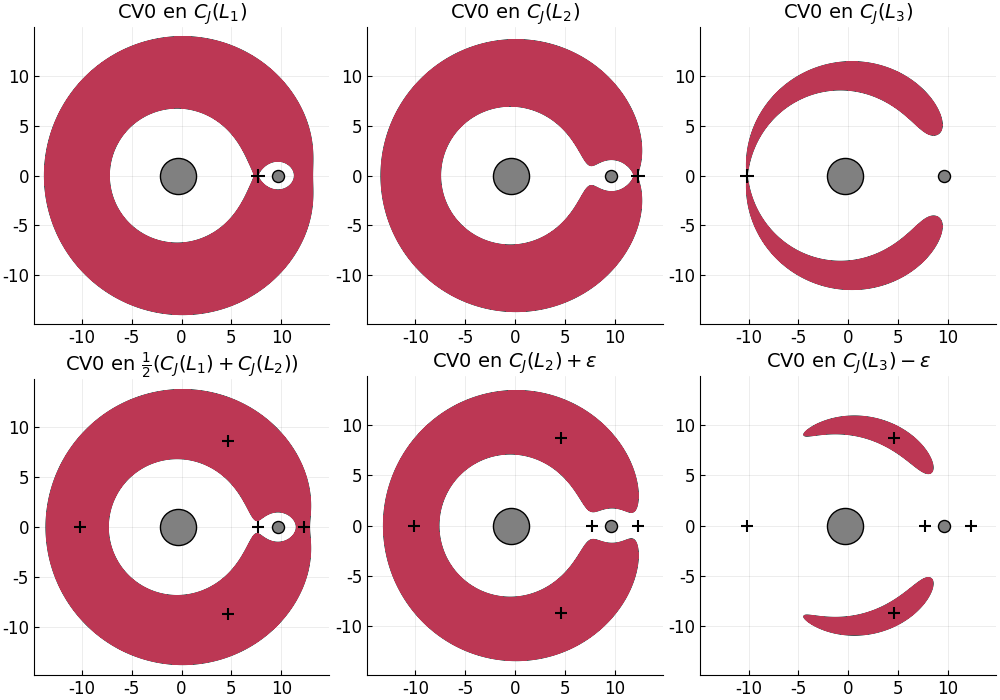
\includegraphics[width=0.9\linewidth]{zero_velocity_curves}
 \caption{\textit{Arriba:} curvas de velocidad cero (CV0) sobre los puntos $L_1, L_2$ y $L_3$, respectivamente. \textit{abajo:} CV0 sobre variaciones en energía sobre las de arriba, se tomó $\varepsilon = 0.05$.}
 \label{fig:zero_velocity_curves}
\end{figure}

La figura \ref{fig:zero_velocity_curves} muestra algunas de estas curvas con consantes de Jacobi alrededor de $L_1$, $L_2$ y $L_3$ y algunas variaciones respecto a estos\footnote{Se graficaron las energías mayores o iguales a la constante de Jacobi para ver la ``sección prohibida'' de las trayectorias.}. Al ser estos puntos tipo silla, dividen al espacio en regiones. El caso más interesantes está entre las energías de $L_1$ y $L_2$, ya que entre éstas se pueden diseñar condiciones iniciales que se queden siempre orbitando entre los dos planetas, o que se quede sólamente en uno de ellos eternamente.

%Falta escoger el segundo problema... esto será después de hacer todos los análisis pertinentes del CR3BP
